% This file is part of the stream_information project.
% Copyright 2017 the authors. All rights reserved.

% # style notes
% - it is Cram\'er--Rao not Cram\'er-Rao. And yet Fisher-matrix not Fisher--matrix.

\documentclass[modern]{aastex61}

% typography
\setlength{\parindent}{1.\baselineskip}
\newcommand{\acronym}[1]{{\small{#1}}}
\newcommand{\CRLB}{\acronym{CRLB}}

% aastex parameters
%%\hypersetup{linkcolor=red,citecolor=green,filecolor=cyan,urlcolor=magenta}
\received{not yet; THIS IS A DRAFT}
%\revised{not yet}
%\accepted{not yet}
%% Adds "Submitted to " the arguement.
%\submitjournal{ApJ}
\shorttitle{information in stellar streams}
\shortauthors{bonaca et al.}

\usepackage{amsmath}

\begin{document}\sloppy\sloppypar\raggedbottom\frenchspacing % trust me

\title{The information content in cold stellar streams}

\correspondingauthor{Ana Bonaca}
% \email{whatevs}

\author[0000-0002-7846-9787]{Ana Bonaca}
\affil{Harvard--Smithsonian Center for Astrophysics}

\author[0000-0003-2866-9403]{David W. Hogg}
\affiliation{Center for Cosmology and Particle Physics,
Department of Physics,
New York University}
\affiliation{Center for Data Science,
New York University}
\affiliation{Flatiron Institute, Simons Foundation}
\affiliation{Max-Planck-Institut f\"ur Astronomie, Heidelberg}

\begin{abstract}\noindent % trust me
Cold stellar streams---produced by tidal disruptions of globular
clusters (or equivalent)---are long-lived, coherent dynamical features
in the stellar halo of the Milky Way.
They have delivered precise information about the mass distribution or
gravitational potential, including constraints on the shape of the
dark-matter halo.
Because of their different positions in phase space, different ages,
and different levels of observational scrutiny, different streams tell
us different things about the Galaxy.
Here we employ a Cram\'er--Rao (\CRLB) or Fisher-matrix approach to
understand the quantitative information content in the known
streams (Pal5, GD-1, Styx, [full list here]).
This approach depends on the existence of a generative model of
stellar streams, which we have developed previously, and which permits
easy calculation of derivatives of predicted stream properties with
respect to Galaxy model parameters.
We find that, in simple, static, analytic models of the Milky Way,
streams XX and YY contain the most information about the dark-matter
shape.
For any individual stream, there are near-degeneracies between
dark-matter halo properties and other parameters, including the mass
of the Large Magellanic Cloud, the total dark-matter mass, and other
potential parameters, but we find that simultaneous fitting of multiple
streams ought to precisely constrain all parameters well.
The \CRLB\ on any one parameter depends strongly on the model freedom;
as we permit more potential freedom, the information about, say, halo
triaxiality, reduces.
We perform experiments to demonstrate this using potential basis
functions that permit great freedom in the gravitational potential on intermediate
scales.
The \CRLB\ formalism also permits us to assess the value of future
measurements of stellar velocities, distances, and proper motions. We
make some comments about the information value of various new
observations that could be made of particular known streams.
\end{abstract}

\keywords{foo --- bar --- hello --- world}

\section{Introduction} \label{sec:intro}

\begin{itemize}
 \item establish streams useful in constraining gravitational potential
 \item tied to parametric models (too complex for inference otherwise, at least in current approaches)
 \item constraints only as good as the model (VL2 results)
 \item so, since not likely that the true potential is NFW, what are the streams constraining? 
 \item here we're building a framework to measure the information content of stellar streams regarding the gravitational potential
 \item two-fold goals: given a simple parametric model, what kind of data do we need? what aspect of a (non-parametric) potential do individual streams constrain?
\end{itemize}


\section{Methods}
\label{sec:method}

\subsection{Information content in stellar streams}
Numerous methods have been developed to estimate properties of a dark matter halo by modeling observations of stellar streams \citep[e.g.,][]{}.
In this approach, the dark matter halo is usually described by an analytic model with a handful of free parameters.
We define the information content in this context as the best-case uncertainties on our model parameters achievable using the observational data at hand.
Formally, the lower bound on the variance of a deterministic parameter is given by the Cram\' er--Rao lower bound \citep[\CRLB,][]{Cramer1946, Rao1945}.

For some data set $\vec{y}$ (e.g., a vector of position and velocity measurements of stars along a stream), the associated covariance matrix is $C_y$.
Given the model parameters $\vec{x}$ (e.g., a vector with the mass and scale radius of a dark matter halo), the Cram\' er--Rao bound is the covariance matrix $C_x$.
The \CRLB\ is set by the inverse of a Fisher information matrix \citep{}:
\begin{equation}
C_x^{-1} = \left(\frac{d\vec{y}}{d\vec{x}}\right)^{T} C_y^{-1} \left(\frac{d\vec{y}}{d\vec{x}}\right)
\label{eq:crlb}
\end{equation}
In the next two subsections, we describe individual terms of Equation~\ref{eq:crlb}: the change in stream observables $\vec{y}$ as a function of changes in the gravitational potential $\vec{x}$, i.e., the derivative $d\vec{y}/d\vec{x}$ (\S\ref{sec:derivatives}), and the adopted observational uncertainties, which set the covariance matrix $C_y$ ( \S\ref{sec:datasets}).

\subsection{Calculating numerical derivatives for the \CRLB}
\label{sec:derivatives}
The variation of observed quantities with the model parameters is the main ingredient when calculating the Cram\' er--Rao bounds.
Stellar streams are characterized by positions and velocities of their member stars, so their observed quantities are the on-sky positions, distances, radial velocities and proper motions.
If we have the present-day position of the stream progenitor, and a representation of the gravitational potential, we can create a forward model of a cold stream.
So, the parameters of our model are a combination of parameters that define the gravitational potential, which are the parameters of interest, and the 6D position of the progenitor, which we treat as hyperparameters.
In what follows, we describe how we measure differences in stream models of different input parameters.

Our model of the gravitational potential is a composite of a Hernquist bulge, a Miyamoto-Nagai disk and a NFW halo.
The fiducial potential is similar to MWPotential2014 \citep{galpy}, which fits a range of observables in the Milky Way, and the used parameters are listed in Table~\ref{t:phi}.
We keep the bulge and disk contributions fixed, and only explore variations induced by changes in the distribution of dark matter.
The dark matter halo is defined by four parameters: two for setting the mass and concentration, and two for the shape of the halo ellipsoid.
To form the streams, we use the following potential form:
\begin{equation}
\begin{aligned}
& \Phi_{dm}(x, y, z) = -V_h^2\, \frac{R_h}{r}\, \ln\left(1 + \frac{r}{R_h}\right) \\
& r^2 = x^2 + \left(\frac{y}{q_y}\right)^2 + \left(\frac{z}{q_z}\right)^2
\end{aligned}
\label{eq:nfw}
\end{equation}
where $V_h$ is the scale velocity, $R_h$ is the scale radius, and $q_y$ and $q_z$ are the $x/y$ and $x/z$ axis ratios, respectively.
In the fiducial potential, the halo is given by $V_h = 430\,\rm km\,s^{-1}$, $R_h = 30\,\rm kpc$, $q_y = q_z = 1$.

- progenitor position today (below described in detail)
- using the streakline method \citep{bonaca}
- timestep: tested time step small enough so that we're not introducing numerical noise that way

\begin{figure}
\begin{center}
\includegraphics[width=\textwidth]{../plots/observable_steps_-1_p0_Ns6.png}
\caption{
}
\label{fig:derivative_steps}
\end{center}
\end{figure}

Figure~\ref{fig:derivative_steps} outlines major steps in our calculation of the numerical derivatives.
We start by creating a pair of stream models, where we change parameter $x_i$ to $x_i = x_{i,0} \pm \Delta x_i$, and keep the rest of the parameters at their fiducial values, $x_j = x_{j,0}$ for $j\neq i$.
The first row of Figure~\ref{fig:derivative_steps} shows models of the GD-1 stream with different offsets $\Delta V_{h}$ from the fiducial scale velocity (color-coded such that the positive offsets are in shades of red, and negative in shades of blue).
Each observable is shown as a function of longitudinal position along the stream, $\xi$, in a separate column in the order from left to right: transverse on-sky position, $\eta$, distance, $d$, radial velocity, $V_r$, and the two proper motion components, $\mu_{\alpha*}$ and $\mu_\delta$.
For each stream, the on-sky positions are rotated to a system in which the great circle best-fitting of the stream track is on the equator.
We describe how we fit these great circles, and provide rotation matrices from the equatorial system to the stream coordinates in Appendix~\ref{}.
Stream models with different scale velocities appear different in all of the observables.
To highlight these differences, we show deviations from the fiducial stream track in the second row.


- the derivative: at fixed stream longitude, $\xi_i$, difference the observable in two models, $\Delta y|_{\xi_i}$.
- regard only transverse direction, as longitudinal has a strong degeneracy with stream age
- noisy data due to the particle nature of streams, interested in a general shape of the stream, so we're fitting a bspline to the stream (more stable than polynomial)
- difference of bsplines from the fiducial for different step sizes in third row
- difference of bsplines divided by the step size in fourth row -- small steps have larger deviations, but these derivatives agree at larger step sizes
To be more robust, we define the derivative of observable $y_i$ with respect to model parameter $x_i$ using symmetrical offsets from the fiducial model:
\begin{equation}
\left.\frac{d y_i}{d x_j}\right\rvert_{\xi_k} = \left.\left(\frac{y_i(x_{0,j} + \Delta x_j) - y_i(x_{0,j} - \Delta x_j)}{2\Delta x_j}\right)\right\rvert_{\xi_k}
\label{eq:derivative}
\end{equation}
for an observation made at the longitudinal position $\xi_k$.
Thus defined derivatives are shown in the last row of Figure~\ref{fig:derivative_steps}, with darker colors corresponding to larger step sizes.
- good agreement

\begin{figure}
\begin{center}
\includegraphics[width=\textwidth]{../plots/step_convergence_-1_halo_progenitor_Ns20_logTrue_l2.png}
\caption{
}
\label{fig:derivative_conv}
\end{center}
\end{figure}

- to quantify whether these have converged
- choice of step size for numerical derivative such that the derivative converged

\subsection{Sets of observational data}
For simplicity, we assume that there are 50 observations uniformly distributed along the length of each stream.


\label{sec:datasets}
\begin{itemize}
 \item fiducial (3D, 4D and 6D)
 \item DESI-like
 \item SDSS-5
 \item Gaia DR2
 \item Gaia final
 \item MM
 \item Gaia final + MM
\end{itemize}

\subsection{Cold tidal streams in the Milky Way}


\section{Results}



\begin{figure}
\begin{center}
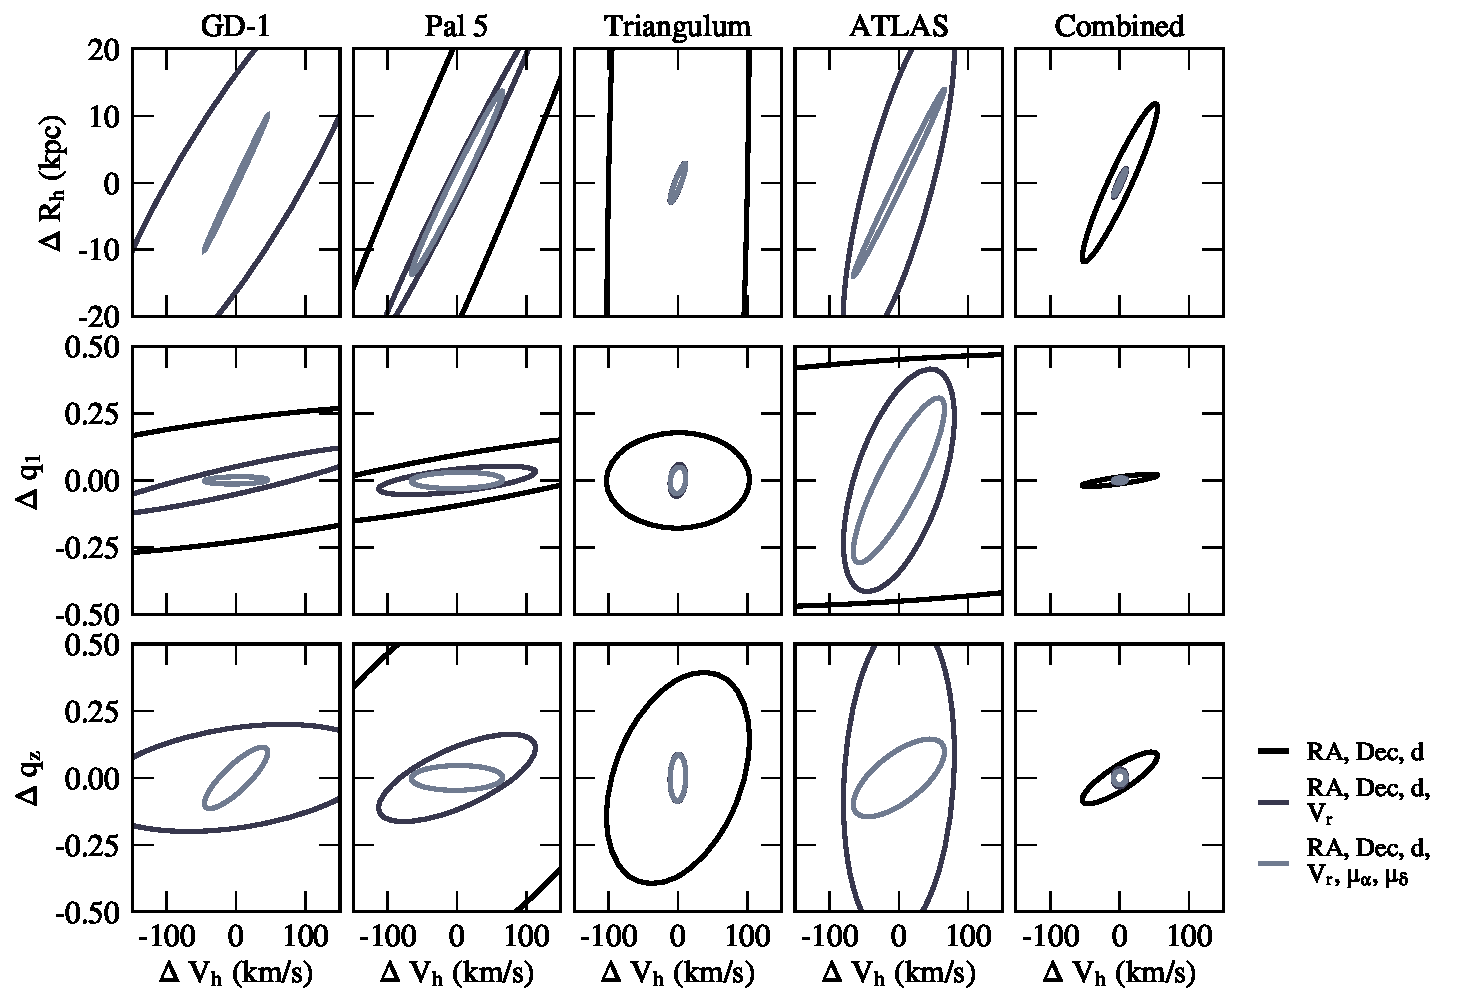
\includegraphics[width=\textwidth]{crlb_2d.pdf}
\caption{Two-dimensional Cram\' er--Rao lower bounds that cold stellar streams put on parameters of the Milky Way dark matter halo.
Parameters considered are the halo scale velocity $V_h$, scale radius $R_h$, $x/y$ and $z/y$ axis ratios $q_1$ and $q_z$, respectively.
Parameter combination is the same across the rows.
Bounds based on individual streams (GD-1, Pal~5, Triangulum and ATLAS) are shown in the first four columns, and their combination is presented in the last column.
The ellipse color denotes the dimensionality of the observational data used to calculate the bound; the darkest ellipses are based on positional information only, medium-colored ellipses include positions and radial velocity, and the lightest ellipses are derived using the full 6-D phase space of streams.
Not all streams are equally constraining for all of the parameters, but for a given stream, parameter constraints improve when more phase-space dimensions are included.
Combining different streams results in the most precise recovery of the halo parameters.
Even if only limited observational data is available for multiple streams, the obtained bounds are comparable to, or better than, the best bounds coming from any individual stream.
}
\label{fig:2dbounds}
\end{center}
\end{figure}

\bibliographystyle{aasjournal}
\bibliography{crlb}

\end{document}

